\begin{task}

\TT{Wyznacz współczynniki zespolonego szeregu Fouriera dla okresowego sygnału $f(t)$ przedstawionego na rysunku}{Calculate coefficients of the periodic signal $f(t)$ shown below for the expansion into a complex exponential Fourier series.} 

\begin{figure}[H]
\centering
\begin{tikzpicture}
  %\draw (0,0) circle (1in);
  \draw[->] (-3.0,+0.0) -- (+5.0,+0.0) node[right] {$t$};
  \draw[->] (+0.0,-1.5) -- (+0.0,+2.0) node[above] {$f(t)$};
  \draw[-,red, thick] (-1.5,0.5) -- (-1.0,1.0) -- (-1.0,0.0) -- (0.0,1.0) -- (0.0,+0.0) -- (+1.0,+1.0) -- (1.0,+1.0) -- (+1.0,+0.0) -- (1.0,+0.0) -- (+2.0,+1.0) -- (+2.0,+0.0) -- (2.5,0.5);
  \draw[-,red, dashed] (-1.5,1.0) -- (2.5,1.0);
  %\draw[-] (-1.0-0.1,-0.1)--(-1.0+0.1,0.1) node[midway, below, outer sep=10pt,align=center] {$-\frac{T}{2}$};
  \draw[-] (-1.0-0.1,-0.1)--(-1.0+0.1,0.1) node[midway, below, outer sep=5pt] {$-T$};
  \draw[-] (+1.0-0.1,-0.1)--(+1.0+0.1,0.1) node[midway, below, outer sep=5pt] {$T$};
  \draw[-] (+2.0-0.1,-0.1)--(+2.0+0.1,0.1) node[midway, below, outer sep=5pt] {$2 \cdot T$};
  \draw[-] (-0.1,+1.0-0.1)--(+0.1,+1.0+0.1) node[midway, left] {$A$};

\end{tikzpicture}
\end{figure}

\TT{W pierwszej kolejności należy ustalić wzór funkcji przedstawionej na rysunku. Jest to funkcja przedziałowa. W pierwszym okresie możemy ja opisać ogólnym równaniem prostej:}{First of all, the definition of $f(t)$ signal has to be derived. This is periodic piecewise function, piecewise linear function to be precise. The simplest form of linear function is:}

\begin{equation}
f(t) = a \cdot t + b
\end{equation}

\TT{W pierwszym okresie wykres funkcji jest prostą przechodzącą przez dwa punkty: $(0,0)$ oraz $(T,A)$. Możemy wiec napisać układ równań rozwiązać go i znaleźć nie znane parametry $a$ i $b$.}{In the first period (i.e. $t \in (0; T)$), linear function crosses two points: $(0,0)$ and $(T,A)$. So, in order to derive $a$ and $b$, the following system of the equations has to be solved.}

\begin{align*}
&\left\{\begin{matrix}
0 = a\cdot 0 +b\\ 
A = a\cdot T +b
\end{matrix}\right. \\
&\left\{\begin{matrix}
0 = b\\ 
A = a\cdot T +b
\end{matrix}\right. \\
&\left\{\begin{matrix}
0 = b\\ 
A = a\cdot T +0
\end{matrix}\right. \\
&\left\{\begin{matrix}
0 = b\\ 
\frac{A}{T} = a
\end{matrix}\right.
\end{align*}

\TT{A więc funkcję przedstawioną na rysunku, w pierwszym okresie można opisać wzorem:}{As a result the piecewise linear function in the first period is given by:}

\begin{align*}
f(t) = \frac{A}{T}\cdot t
\end{align*}

\TT{I ogólniej całą funkcję można wyrazić następującym wzorem}{For the whole periodic signal $f(t)$ we get:}

\begin{align*}
f(t) = \begin{matrix}\frac{A}{T}\cdot \left(t-k\cdot T\right) & t \in \left ( 0+k \cdot T; T + k \cdot T \right )\wedge k \in \TT{C}{Z}\end{matrix}
\end{align*}

\TT{Współczynnik $F_0$ wyznaczamy ze wzoru:}{The $F_0$ coefficient is defined as:}

\begin{equation}
F_0=\frac{1}{T}\int_{T}f(t) \cdot dt
\end{equation}

\TT{Podstawiamy do wzoru wzór naszej funkcji w pierwszym okresie $k=0$}{For the period $t \in (0; T)$, i.e. $k=0$, we get:}

\begin{align*}
F_0&=\frac{1}{T}\int_{T}f(t) \cdot dt=\\
&=\frac{1}{T}\int_{0}^{T} \frac{A}{T}\cdot t \cdot dt=\\
&=\frac{A}{T^2}\int_{0}^{T} t \cdot dt=\\
&=\frac{A}{T^2}\cdot \left. \frac{1}{2}\cdot t^2 \right|_{0}^{T}=\\
&=\frac{A}{T^2}\cdot \frac{1}{2}\cdot \left( T^2 -0^2 \right)=\\
&=\frac{A}{T^2}\cdot \frac{1}{2}\cdot T^2=\\
&=\frac{A}{2}
\end{align*}

\TT{Wartość współczynnika $F_0$ wynosi $\frac{A}{2}$.}{The $F_0$ coefficient equals $\frac{A}{2}$.}

\TT{Współczynniki $F_k$ wyznaczamy ze wzoru}{The $F_k$ coefficients are defined as:}

\begin{equation}
F_k=\frac{1}{T}\int_{T}f(t) \cdot e^{ -\jmath \cdot k \cdot \frac{2\pi}{T} \cdot t} \cdot dt
\end{equation}

\TT{Podstawiamy do wzoru wzór naszej funkcji w pierwszym okresie $k=0$}{For the period $t \in (0; T)$, i.e. $k=0$, we get:}

\begin{align*}
F_k&=\frac{1}{T}\int_{T}f(t) \cdot e^{ -\jmath \cdot k \cdot \frac{2\pi}{T} \cdot t} \cdot dt=\\
&=\frac{1}{T}\int_{0}^{T} \frac{A}{T} \cdot t \cdot e^{ -\jmath \cdot k \cdot \frac{2\pi}{T} \cdot t} \cdot dt=\\
&=\frac{1\cdot A}{T^2}\int_{0}^{T} t \cdot e^{ -\jmath \cdot k \cdot \frac{2\pi}{T} \cdot t} \cdot dt=\\
&=\begin{Bmatrix*}[l]
u&=t & dv&=e^{ -\jmath \cdot k \cdot \frac{2\pi}{T} \cdot t} \cdot dt \\
du&=dt & v&=\frac{T}{-\jmath \cdot k\cdot 2\pi}\cdot e^{ -\jmath \cdot k \cdot \frac{2\pi}{T} \cdot t}
\end{Bmatrix*}=\\
&=\frac{A}{T^2}\cdot \left( \left. t \cdot \frac{T}{-\jmath \cdot k\cdot 2\pi}\cdot e^{ -\jmath \cdot k \cdot \frac{2\pi}{T} \cdot t} \right|_{0}^{T} - \int_{0}^{T}  \frac{T}{-\jmath \cdot k\cdot 2\pi}\cdot e^{ -\jmath \cdot k \cdot \frac{2\pi}{T} \cdot t} \cdot dt \right)=\\
&=\frac{A}{T^2}\cdot \left( \left( T \cdot \frac{T}{-\jmath \cdot k\cdot 2\pi}\cdot e^{ -\jmath \cdot k \cdot \frac{2\pi}{T} \cdot T} - 0 \cdot \frac{T}{-\jmath \cdot k\cdot 2\pi}\cdot e^{ -\jmath \cdot k \cdot \frac{2\pi}{T} \cdot 0} \right) + \left.  \frac{T^2}{\left(-\jmath \cdot k\cdot 2\pi\right)^2}\cdot e^{ -\jmath \cdot k \cdot \frac{2\pi}{T} \cdot t} \right|_{0}^{T} \right)=\\
&=\frac{A}{T^2}\cdot \left(\frac{T^2}{-\jmath \cdot k\cdot 2\pi}\cdot e^{ -\jmath \cdot k \cdot \frac{2\pi}{T} \cdot T} + \frac{T^2}{- \left(k\cdot 2\pi\right)^2}\cdot \left( e^{ -\jmath \cdot k \cdot \frac{2\pi}{T} \cdot T} - e^{ -\jmath \cdot k \cdot \frac{2\pi}{T} \cdot 0} \right) \right)=\\
&=A\cdot \left(\frac{1}{-\jmath \cdot k\cdot 2\pi}\cdot e^{ -\jmath \cdot k \cdot 2\pi} - \frac{1}{\left(k\cdot 2\pi\right)^2}\cdot \left(e^{ -\jmath \cdot k \cdot 2\pi} -e^{ 0} \right) \right)=\\
&=A\cdot \left(\frac{1}{-\jmath \cdot k\cdot 2\pi} - \frac{1}{\left(k\cdot 2\pi\right)^2}\cdot \left( 1 - 1 \right) \right)=\\
&=A\cdot \left(\frac{1}{-\jmath \cdot k\cdot 2\pi} - \frac{1}{\left(k\cdot 2\pi\right)^2}\cdot 0 \right)=\\
&=A\cdot \left(\frac{1}{-\jmath \cdot k\cdot 2\pi} - 0\right)=\\
&=\frac{A}{-\jmath \cdot k\cdot 2\pi}=\\
&=\jmath \cdot \frac{A}{k\cdot 2\pi}
\end{align*}

\TT{Wartość współczynnika $F_k$ wynosi $\jmath \cdot \frac{A}{k\cdot 2\pi}$.}{The $F_k$ coefficients equal to $\jmath \cdot \frac{A}{k\cdot 2\pi}$.}

\TT{Ostatecznie współczynniki zespolonego szeregu Fouriera dla funkcji przedstawionej na rysunku przyjmują wartości.}{To sum up, coefficients for the expansion into a complex exponential Fourier series are given by:}

\begin{align*}
F_0&=\frac{A}{2}\\
F_k&=\jmath \cdot \frac{A}{k\cdot 2\pi}\\
\end{align*}

\TT{Możemy wyznaczyć kilka wartości współczynników $F_k$}{The first several coefficients are equal to:}

\begin{table}[H]
  \centering  
  \begin{tabular}{|c|c|c|c|c|c|c|c|c|c|c|c|}
    \hline 
    $k$ & $-5$ & $-4$ & $-3$ & $-2$ & $-1$ & $0$ & $1$ & $2$ & $3$ & $4$ & $5$\\ 
    \hline 
    $F_k$ & $-\jmath\cdot \frac{A}{10\cdot \pi}$ & $-\jmath\cdot \frac{A}{8\cdot \pi}$ & $-\jmath\cdot \frac{A}{6\cdot \pi}$ & $-\jmath\cdot \frac{A}{4\cdot \pi}$ & $-\jmath\cdot \frac{A}{2\cdot \pi}$ & $\frac{A}{2}$ & $\jmath\cdot \frac{A}{2\cdot \pi}$ & $\jmath\cdot \frac{A}{4\cdot \pi}$ & $\jmath\cdot \frac{A}{6\cdot \pi}$ & $\jmath\cdot \frac{A}{8\cdot \pi}$ & $\jmath\cdot \frac{A}{10\cdot \pi}$\\ 
    \hline 
    $\left|F_k\right|$ & $\frac{A}{10\cdot \pi}$ & $\frac{A}{8\cdot \pi}$ & $\frac{A}{6\cdot \pi}$ & $\frac{A}{4\cdot \pi}$ & $\frac{A}{2\cdot \pi}$ & $\frac{A}{2}$ & $\frac{A}{2\cdot \pi}$ & $\frac{A}{4\cdot \pi}$ & $\frac{A}{6\cdot \pi}$ & $\frac{A}{8\cdot \pi}$ & $\frac{A}{10\cdot \pi}$\\ 
    \hline 
    $Arg\left(F_k\right)$ & $-\frac{\pi}{2}$ & $-\frac{\pi}{2}$ & $-\frac{\pi}{2}$ & $-\frac{\pi}{2}$ & $-\frac{\pi}{2}$ & $0$ & $\frac{\pi}{2}$ & $\frac{\pi}{2}$ & $\frac{\pi}{2}$ & $\frac{\pi}{2}$ & $\frac{\pi}{2}$\\ 
    \hline 
  \end{tabular} 
\end{table}

\TT{Podstawiając to wzoru aproksymacyjnego funkcje $f(t)$ możemy wyrazić jako}{Hence, the signal $f(t)$ may be expressed as the sum of the harmonic series}

\begin{equation}
\begin{aligned}
f(t) &= \sum_{k=-\infty}^{\infty} F_k \cdot e^{\jmath \cdot k \cdot \frac{2\pi}{T} \cdot t}\\
f(t) &= \frac{A}{2} + \sum_{\begin{smallmatrix}k=-\infty \\ k \neq 0 \end{smallmatrix}}^{\infty} \left[\jmath \cdot \frac{A}{k\cdot 2\pi}\right] \cdot e^{\jmath \cdot k \cdot \frac{2\pi}{T} \cdot t}
\end{aligned}
\end{equation}

\TT{W przypadku sumowania od $k_{min}=-1$ do $k_{max}=1$ otrzymujemy:}{A partial approximation of the $f(t)$ signal from $k_{min}=-1$ to $k_{max}=1$ results in:}

\begin{figure}[H]
  \centering
  \begin{tikzpicture}
  %\draw (0,0) circle (1in);
  \draw[->] (-3.0,+0.0) -- (+5.0,+0.0) node[right] {$t$};
  \draw[->] (+0.0,-1.5) -- (+0.0,+1.5) node[above] {$f(t)$};
  %\draw[-,red, thick] (-2.5,+0.0) -- (+0.0,+0.0);
  %\draw[-] (-1.0-0.1,-0.1)--(-1.0+0.1,0.1) node[midway, below, outer sep=10pt,align=center] {$-\frac{T}{2}$};
  \draw[-] (-2.0-0.1,-0.1)--(-2.0+0.1,0.1) node[midway, below, outer sep=5pt,align=center] {$-T$};
  \draw[-] (+4.0-0.1,-0.1)--(+4.0+0.1,0.1) node[midway, below, outer sep=5pt] {$2 \cdot T$};
  \draw[-] (+2.0-0.1,-0.1)--(+2.0+0.1,0.1) node[midway, below, outer sep=5pt] {$T$};
  \draw[-] (-0.1,1.0-0.1)--(+0.1,1.0+0.1) node[midway, right] {$A$};
  
  \draw[scale=1.0,domain=-2.5:4.5,samples=100,smooth,variable=\x,red,thick] plot ({\x},{0.5-1.0/3.141592*sin(\x*180.0/3.141592*1*3.141592/1.0)});
  \end{tikzpicture}
\end{figure}

\TT{W przypadku sumowania od $k_{min}=-2$ do $k_{max}=2$ otrzymujemy:}{A partial approximation of the $f(t)$ signal from $k_{min}=-2$ to $k_{max}=2$ results in:}

\begin{figure}[H]
  \centering
  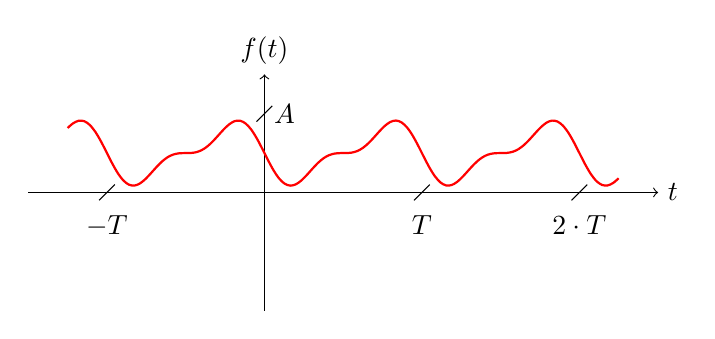
\begin{tikzpicture}
  %\draw (0,0) circle (1in);
  \draw[->] (-3.0,+0.0) -- (+5.0,+0.0) node[right] {$t$};
  \draw[->] (+0.0,-1.5) -- (+0.0,+1.5) node[above] {$f(t)$};
  %\draw[-,red, thick] (-2.5,+0.0) -- (+0.0,+0.0);
  %\draw[-] (-1.0-0.1,-0.1)--(-1.0+0.1,0.1) node[midway, below, outer sep=10pt,align=center] {$-\frac{T}{2}$};
  \draw[-] (-2.0-0.1,-0.1)--(-2.0+0.1,0.1) node[midway, below, outer sep=5pt,align=center] {$-T$};
  \draw[-] (+4.0-0.1,-0.1)--(+4.0+0.1,0.1) node[midway, below, outer sep=5pt] {$2 \cdot T$};
  \draw[-] (+2.0-0.1,-0.1)--(+2.0+0.1,0.1) node[midway, below, outer sep=5pt] {$T$};
  \draw[-] (-0.1,1.0-0.1)--(+0.1,1.0+0.1) node[midway, right] {$A$};
  
  \draw[scale=1.0,domain=-2.5:4.5,samples=100,smooth,variable=\x,red,thick] plot ({\x},{0.5-1.0/3.141592*sin(\x*180.0/3.141592*1*3.141592/1.0)-1.0/(2*3.141592)*sin(\x*180.0/3.141592*2*3.141592/1.0)});
  \end{tikzpicture}
\end{figure}

\TT{W przypadku sumowania od $k_{min}=-3$ do $k_{max}=3$ otrzymujemy:}{A partial approximation of the $f(t)$ signal from $k_{min}=-3$ to $k_{max}=3$ results in:} 

\begin{figure}[H]
  \centering
  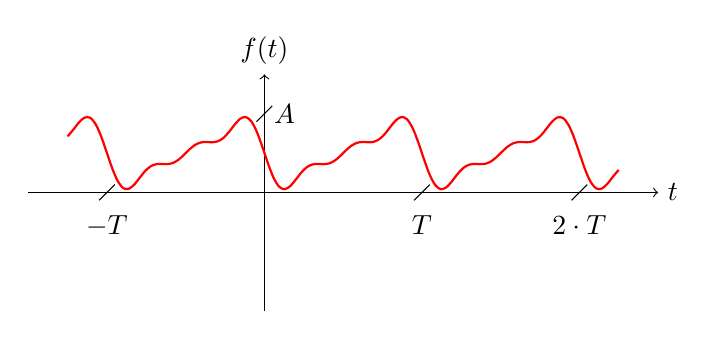
\begin{tikzpicture}
  %\draw (0,0) circle (1in);
  \draw[->] (-3.0,+0.0) -- (+5.0,+0.0) node[right] {$t$};
  \draw[->] (+0.0,-1.5) -- (+0.0,+1.5) node[above] {$f(t)$};
  %\draw[-,red, thick] (-2.5,+0.0) -- (+0.0,+0.0);
  %\draw[-] (-1.0-0.1,-0.1)--(-1.0+0.1,0.1) node[midway, below, outer sep=10pt,align=center] {$-\frac{T}{2}$};
  \draw[-] (-2.0-0.1,-0.1)--(-2.0+0.1,0.1) node[midway, below, outer sep=5pt,align=center] {$-T$};
  \draw[-] (+4.0-0.1,-0.1)--(+4.0+0.1,0.1) node[midway, below, outer sep=5pt] {$2 \cdot T$};
  \draw[-] (+2.0-0.1,-0.1)--(+2.0+0.1,0.1) node[midway, below, outer sep=5pt] {$T$};
  \draw[-] (-0.1,1.0-0.1)--(+0.1,1.0+0.1) node[midway, right] {$A$};
  
  \draw[scale=1.0,domain=-2.5:4.5,samples=100,smooth,variable=\x,red,thick] plot ({\x},{0.5-1.0/3.141592*sin(\x*180.0/3.141592*1*3.141592/1.0)-1.0/(2*3.141592)*sin(\x*180.0/3.141592*2*3.141592/1.0)-1.0/(3*3.141592)*sin(\x*180.0/3.141592*3*3.141592/1.0)});
  \end{tikzpicture}
\end{figure}

\TT{W przypadku sumowania od $k_{min}=-7$ do $k_{max}=7$ otrzymujemy:}{A partial approximation of the $f(t)$ signal from $k_{min}=-7$ to $k_{max}=7$ results in:}

\begin{figure}[H]
  \centering
  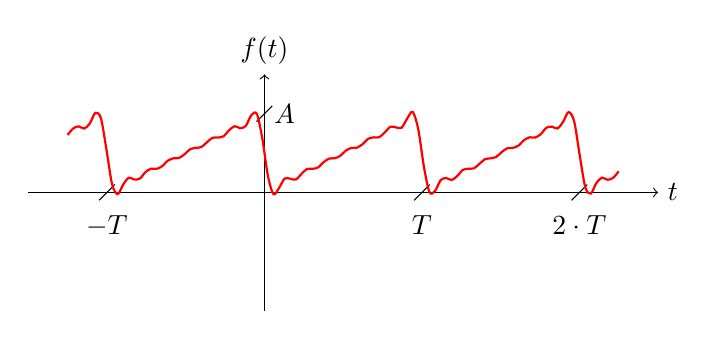
\begin{tikzpicture}
  %\draw (0,0) circle (1in);
  \draw[->] (-3.0,+0.0) -- (+5.0,+0.0) node[right] {$t$};
  \draw[->] (+0.0,-1.5) -- (+0.0,+1.5) node[above] {$f(t)$};
  %\draw[-,red, thick] (-2.5,+0.0) -- (+0.0,+0.0);
  %\draw[-] (-1.0-0.1,-0.1)--(-1.0+0.1,0.1) node[midway, below, outer sep=10pt,align=center] {$-\frac{T}{2}$};
  \draw[-] (-2.0-0.1,-0.1)--(-2.0+0.1,0.1) node[midway, below, outer sep=5pt,align=center] {$-T$};
  \draw[-] (+4.0-0.1,-0.1)--(+4.0+0.1,0.1) node[midway, below, outer sep=5pt] {$2 \cdot T$};
  \draw[-] (+2.0-0.1,-0.1)--(+2.0+0.1,0.1) node[midway, below, outer sep=5pt] {$T$};
  \draw[-] (-0.1,1.0-0.1)--(+0.1,1.0+0.1) node[midway, right] {$A$};
  
  \draw[scale=1.0,domain=-2.5:4.5,samples=100,smooth,variable=\x,red,thick] plot ({\x},{0.5-1.0/3.141592*sin(\x*180.0/3.141592*1*3.141592/1.0)-1.0/(2*3.141592)*sin(\x*180.0/3.141592*2*3.141592/1.0)-1.0/(3*3.141592)*sin(\x*180.0/3.141592*3*3.141592/1.0)-1.0/(4*3.141592)*sin(\x*180.0/3.141592*4*3.141592/1.0)-1.0/(5*3.141592)*sin(\x*180.0/3.141592*5*3.141592/1.0)-1.0/(6*3.141592)*sin(\x*180.0/3.141592*6*3.141592/1.0)-1.0/(7*3.141592)*sin(\x*180.0/3.141592*7*3.141592/1.0)});
  \end{tikzpicture}
\end{figure}

\TT{W przypadku sumowania od $k_{min}=-11$ do $k_{max}=11$ otrzymujemy:}{A partial approximation of the $f(t)$ signal from $k_{min}=-11$ to $k_{max}=11$ results in:} 

\begin{figure}[H]
  \centering
  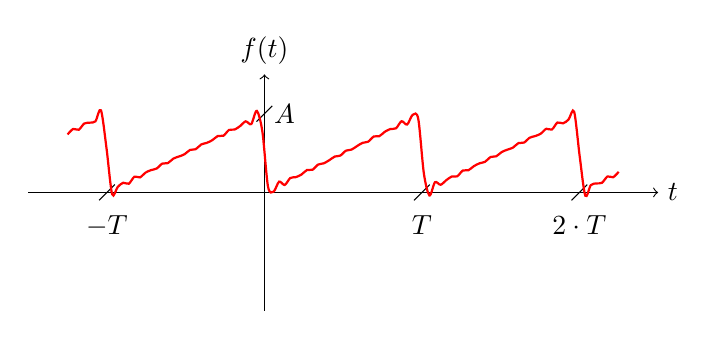
\begin{tikzpicture}
  %\draw (0,0) circle (1in);
  \draw[->] (-3.0,+0.0) -- (+5.0,+0.0) node[right] {$t$};
  \draw[->] (+0.0,-1.5) -- (+0.0,+1.5) node[above] {$f(t)$};
  %\draw[-,red, thick] (-2.5,+0.0) -- (+0.0,+0.0);
  %\draw[-] (-1.0-0.1,-0.1)--(-1.0+0.1,0.1) node[midway, below, outer sep=10pt,align=center] {$-\frac{T}{2}$};
  \draw[-] (-2.0-0.1,-0.1)--(-2.0+0.1,0.1) node[midway, below, outer sep=5pt,align=center] {$-T$};
  \draw[-] (+4.0-0.1,-0.1)--(+4.0+0.1,0.1) node[midway, below, outer sep=5pt] {$2 \cdot T$};
  \draw[-] (+2.0-0.1,-0.1)--(+2.0+0.1,0.1) node[midway, below, outer sep=5pt] {$T$};
  \draw[-] (-0.1,1.0-0.1)--(+0.1,1.0+0.1) node[midway, right] {$A$};
  
  \draw[scale=1.0,domain=-2.5:4.5,samples=100,smooth,variable=\x,red,thick] plot ({\x},{0.5-1.0/3.141592*sin(\x*180.0/3.141592*1*3.141592/1.0)-1.0/(2*3.141592)*sin(\x*180.0/3.141592*2*3.141592/1.0)-1.0/(3*3.141592)*sin(\x*180.0/3.141592*3*3.141592/1.0)-1.0/(4*3.141592)*sin(\x*180.0/3.141592*4*3.141592/1.0)-1.0/(5*3.141592)*sin(\x*180.0/3.141592*5*3.141592/1.0)-1.0/(6*3.141592)*sin(\x*180.0/3.141592*6*3.141592/1.0)-1.0/(7*3.141592)*sin(\x*180.0/3.141592*7*3.141592/1.0)-1.0/(8*3.141592)*sin(\x*180.0/3.141592*8*3.141592/1.0)-1.0/(9*3.141592)*sin(\x*180.0/3.141592*9*3.141592/1.0)-1.0/(10*3.141592)*sin(\x*180.0/3.141592*10*3.141592/1.0)-1.0/(11*3.141592)*sin(\x*180.0/3.141592*11*3.141592/1.0)});
  \end{tikzpicture}
\end{figure}

\TT{W granicy sumowania od $k_{min}=-\infty$ do $k_{max}=\infty$ otrzymujemy oryginalny sygnał.}{Approximation of the $f(t)$ signal for from $k_{min}=-\infty$ to $k_{max}=\infty$ results in oryginal signal.}

\end{task}